\documentclass{article}
\usepackage[T1]{fontenc}
\usepackage[portuguese]{babel}
\usepackage{amsfonts}
\usepackage{amsmath}
\usepackage{hyperref}
\usepackage{graphicx}
\usepackage{bm}
\usepackage{chemfig}
\usepackage{hyperref}
\usepackage{listings}
\usepackage[a4paper,margin=2cm]{geometry}

% Adiciona a parte de bibliografia
\usepackage{biblatex}
\addbibresource{exemplo.bib}

\begin{document}

\section{Dados para estes exemplos}
Documento da classe \textit{article}, com margens de $2cm$ em uma folha $A4$. Vamos precisar dos pacotes 
%
% lslisting serve para colocar código de programas no LaTeX. Não utilizar acentos dentro deste ambiente...depois explico como colocar acentos.
%
\begin{lstlisting}
\documentclass{article}
\usepackage[T1]{fontenc}
\usepackage[portuguese]{babel}
\usepackage{amsfonts}
\usepackage{amsmath}
\usepackage{graphicx}
\usepackage{bm}
\usepackage{chemfig}
\usepackage{listings}
\usepackage[a4paper,margin=2cm]{geometry}
\usepackage{biblatex}
\addbibresource{exemplo.bib}
\end{lstlisting}
\section{Integração}
Todos sabemos que a integração pode ser entendida como o limite de uma soma com infinitos termos
\begin{equation}\label{eq:1}
    \int_a^b f(x) \,dx = \lim_{\Delta x \to 0} \sum_{i=1}^\infty f(x_i)\Delta x, \quad x \in [a,b].
\end{equation}

A expressão da Equação \ref{eq:1} pode ser calculada de forma aproximada com o método dos retângulos
\begin{equation}\label{eq:retangulos}
    \int_a^b f(x) \,dx \approx  \sum_{i=1}^N f(x_i)\Delta x, \quad x_i = a + (i-1)\Delta x ,
\end{equation}
em que $\Delta x = \frac{b-a}{N}$. A interpretação geométrica da aproximação pode ser visualizada na Figura \ref{fig:retangulos}, para $N=8$.

\begin{figure}[h!]
    \centering
    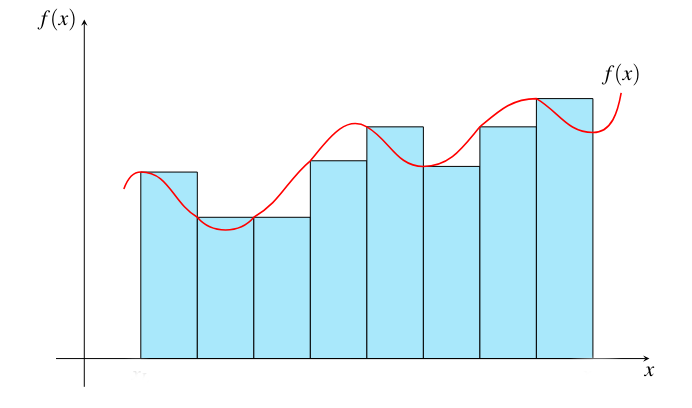
\includegraphics[width=0.5\linewidth]{retangulos.png}
    \caption{Aproximação do valor da integral pelo método dos retângulos}
    \label{fig:retangulos}
\end{figure}
\section{Sistemas de Equações Lineares}
Todos sabemos, também, que um sistema de equações lineares
%
% Aqui tem uma coisa interessante. Queremos chaves do lado esquerdo da equação mas não no lado direito. Como em TeX sempre temos que fechar o que foi aberto, podemos usar \right . para fechar sem colocar um símbolo. Então, o \left \lbrace vai abrir uma chave para a esquerda (l é left e brace é chaves). Seguindo a mesma lógia, temos o comando \rbrace também. 
%
\begin{equation}
    \left \lbrace
    \begin{array}{ccc}
    3x + y & = &4 \\
    x + 2y & = & 2
    \end{array}
    \right .
\end{equation}
pode ser escrito na forma matricial
%
% O bmatrix cria  um array com [ ] e o Bmatrix com {}. 
%
\begin{equation}\label{eq:sistema}
    \begin{bmatrix}
        3 & 1 \\
        1 & 2
    \end{bmatrix}\begin{Bmatrix}
        x \\
        y
    \end{Bmatrix} = \begin{Bmatrix}
        4 \\
        2
    \end{Bmatrix},
\end{equation}
ou 
\begin{equation}
    \mathbf{A}\mathbf{x}=\mathbf{b}.
\end{equation}
O sistema linear da Eq. \ref{eq:sistema} tem solução dada por
\begin{equation}
    \mathbf{x}=\mathbf{A}^{-1}\mathbf{b}.
\end{equation}
\section{Um pouco de química}
Outro assunto de conhecimento comum é que todo o estudante de exatas precisa de café. Neste caso, podemos utilizar o pacote \textit{chemfig} para impressionar os colegas, gerando a imagem da Figura \ref{fig:cafeina}. Uma boa introdução ao pacote de química pode ser encontrado em \href{https://www.overleaf.com/learn/latex/Chemistry_formulae}{https://www.overleaf.com/learn/latex/Chemistry\_formulae}
%
% Para colocar o link acima usamos o pacote hyperef. Observe que o TeX, sempre que encontrar um _ no texto, vai colocar o próximo símbolo para baixo (sub escrito). Por isso, eu coloquei um \ antes do _formulae no texto do hyperlink (não no endereço, que iria dar problema ao acessar o link)
%



\begin{figure}[h!]
    \centering
\chemfig{*6((=O)-N(-)-(*5(-N=-N(-)-))=-(=O)-N(-)-)}    
    \caption{Molécula de cafeína $C_8H_{10}N_4O_2$}
    \label{fig:cafeina}
\end{figure}

\section{Brincando um pouco com símbolos}

O uso de símbolos no \LaTeX é bem intuitivo. Por exemplo, os comandos
\begin{lstlisting}
\begin{equation*}
    \Omega \, \omega
\end{equation*}
\end{lstlisting}
resulta em 
\begin{equation*}
    \Omega \, \omega
\end{equation*}

Um cuidado que temos que ter com símbolos em negrito é que precisamos do pacote \textit{bm}

\begin{lstlisting}
\begin{equation*}
    \bm{\Omega} \, \bm{\omega}
\end{equation*}
\end{lstlisting}
resulta em 
\begin{equation*}
    \bm{\Omega} \, \bm{\omega}
\end{equation*}

Para letras 'normais' podemos usar o comando
\begin{lstlisting}
    \mathbf{O}
\end{lstlisting}
resultando em 
\begin{equation*}
    \mathbf{O}
\end{equation*}

Outros comandos bem úteis são  o \textit{mathbb} e o \textit{mathcal}

\begin{equation*}
  \text{mathbb}:  \mathbb{N}, \mathbb{R}, \mathbb{Z}
\end{equation*}
e
\begin{equation*}
  \text{mathcal}:  \mathcal{N}, \mathcal{R}, \mathcal{Z}
\end{equation*}

\section{Referências}

Citando então o \cite{nomefacil1} e também o \cite{nomefacil2}

\printbibliography

\end{document}